 % !TEX encoding = UTF-8 Unicode

\documentclass[a4paper]{article}

\usepackage{color}
\usepackage{url}
\usepackage[T2A]{fontenc} % enable Cyrillic fonts
\usepackage[utf8]{inputenc} % make weird characters work
\usepackage{graphicx}

\usepackage[english,serbian]{babel}
%\usepackage[english,serbianc]{babel} %ukljuciti babel sa ovim opcijama, umesto gornjim, ukoliko se koristi cirilica

\usepackage[unicode]{hyperref}
\hypersetup{colorlinks,citecolor=green,filecolor=green,linkcolor=blue,urlcolor=blue}

%\newtheorem{primer}{Пример}[section] %ćirilični primer
\newtheorem{primer}{Primer}[section]

\begin{document}

\title{Sajber rat\\ \small{Seminarski rad u okviru kursa\\Racunarstvo i drustvo\\ Matematički fakultet}}

\author{Luka Vukotic\\ mi19120@alas.matf.bg.ac.rs}
\date{24.~maj 2022.}
\maketitle

\abstract{
U ovom radu su objasnjeni pojmovi vezani za sajber rat i sve vezano za sam ovaj pojam

\tableofcontents

\newpage

\section{Uvod}
\label{sec:uvod}
Sajber rat je potajan i nevidljiv za vecinu. Naime on se odvija u sajber prostoru koga cine sve racunarske mreze na svetu. \textbf{Sajber-prostor} se cesto definise i kao peto ratno podrucje posle kopna, mora,vazduha i svemira za koje si vec znamo.
Termin sajber rata je koriscen u mnogim razlicitim kontekstima, ali u vecini slucajeva sa sobom ne povlaci neki vid nasija na koji smo kroz istoriju navikli kada pomenemo samu rec rat. Sajber rat moze ukljucivati kineticke i nekineticke aktivnosti:
\begin{itemize}
\item Pod pojmom kineticke aktivnosti mislimo na aktivnosti koje se povezuju sa nekim vidom kretanja(npr. pokretanje vojnih snaga, bacanje bombi i koriscenje vojnog naoruzanja u nekom podrucju)
\item Nekineticke aktivnosti su uglavnom usmerene ka bilo kom pristupu suparnickim sajber sistemima, kao sto su prisluskivanje, preuzimanje obavestajnih podataka itd...
\end{itemize} 

\section{Sta je sajber rat?}
Sto se tice neke univerzalne definicije ona jos uvek ne postoji.
Naime, postoji znacajna debata medju ekspertima u ovoj oblasti o definiciji pojma sajber rata/ratovanja kao i da li tako nesto uopste postoji. Postoji tu dosta prolema koji se javljaju prilikom pronalazenja univerzalne definicije.
Prvi problem prilikom definisanja ovog pojma je to sto sajber ratovanje ne ispunjava tipicnu definiciju rata, ali ipak mnoge drzave imaju aktivne sajber operacije za napad i odbranu. Pored vec pomenutih problema, eksponencijalni rast inetrneta i internet tehnologija dovodi do toga da sajber napadi budu sve rasprostranjeniji, i u ovakvom okruzenju uticaj zakona o sajber ratovanju moze biti veoma ogranicen.
Ipak iako ne postoji prihvacena univerzalna definicija postoji vise razlicitih definicija koje mogu biti kandidati:
\begin{itemize}
\item  Talinski prirucnik definise sajber rat kao sajber napad, u
odbranbenoj ili napadnoj sajber operaciji, koji rezultuje u
nasilju, smrti i/ili destrukciji. Nedostatak ove definicije -
iskljucuje npr. sajber operacije dizajnirane da destabilizuju
finansijski sistem nacionalne drzave
\item DCAF odnosno zenevski centar za demokratsku kontrolu oruzanih snaga je usvojio sledecu definiciju:sajber rat je ratno ponasanje koje se sprovodi u virtuelnom svetu koristeci informacije, komunikacionu tehnologiju i mreze, sa namerom da poremeti ili unisti neprijateljske informacione i komunikacione sisteme
\end{itemize} 




\section{Ucestalost sajber napada}	
\label{sec:termini_i_citiranje}

Sto se tice ucestalosti sajber napada prakticno je nemoguce identifikovati/detektovati svaki sajber napad koji se dogodi.
Neki napadi se mogu neopazeno odvijati godinama (veoma napredan sistem), drugi su kratkotrajni ali za sobom ne ostavljaju stragove pomocu kojih bi mogli biti otkriveni.
Takodje problem pravi i razvoj same tehnologije jer se sa razvojem povecava broj napada kao i njihova raznovrsnost, ali jedna od dobrih stvari je ta sto se poboljsavaju i odbrambeni mehanizmi kao i sistemi za detekciju napada.  
Deutsche Telekom AG (DTAG), nemacka kompanija za telekomunikacije, uspostavila je mrezu od 97 senzora koji
sluze kao sistem ranog upozorenja koji će u realnom vremenu przžiti sliku o tekucem sajber napadima. 
Iako je vecina senzora smestena u Nemackoj, DTAG takodje locira honeypots\footnote{Honeypot je racunarski sigurnosni mehanizam postavljen za otkrivanje, uklanjanje ili, na neki nacin, suzbijanje pokusaja neovlasćene upotrebe informacionih sistema.
} 
i senzore u drugim neevropskim zemljama.
\newline
Top petnaest zemalja koje su DTAG senzori zabelezili kao izvor sajber napada istaknuti su na slici 1. 
Otprilike 20\% navedenih sajber napada bilo je poreklom iz Ruske Federacije. 
Prve cetiri navedene drzave, ukljucujuci SAD, Nemacku i Tajvan, cinile su 62\% zastupljenih sajber napada.
Ovi slucajevi pruzaju sliku napada usmerenih na odredjeno geografsko podrucje, u ovom slucaju Evropu.
 


\begin{verbatim}
\end{verbatim}

\begin{figure}[h!]
  \centering
  \begin{center}
  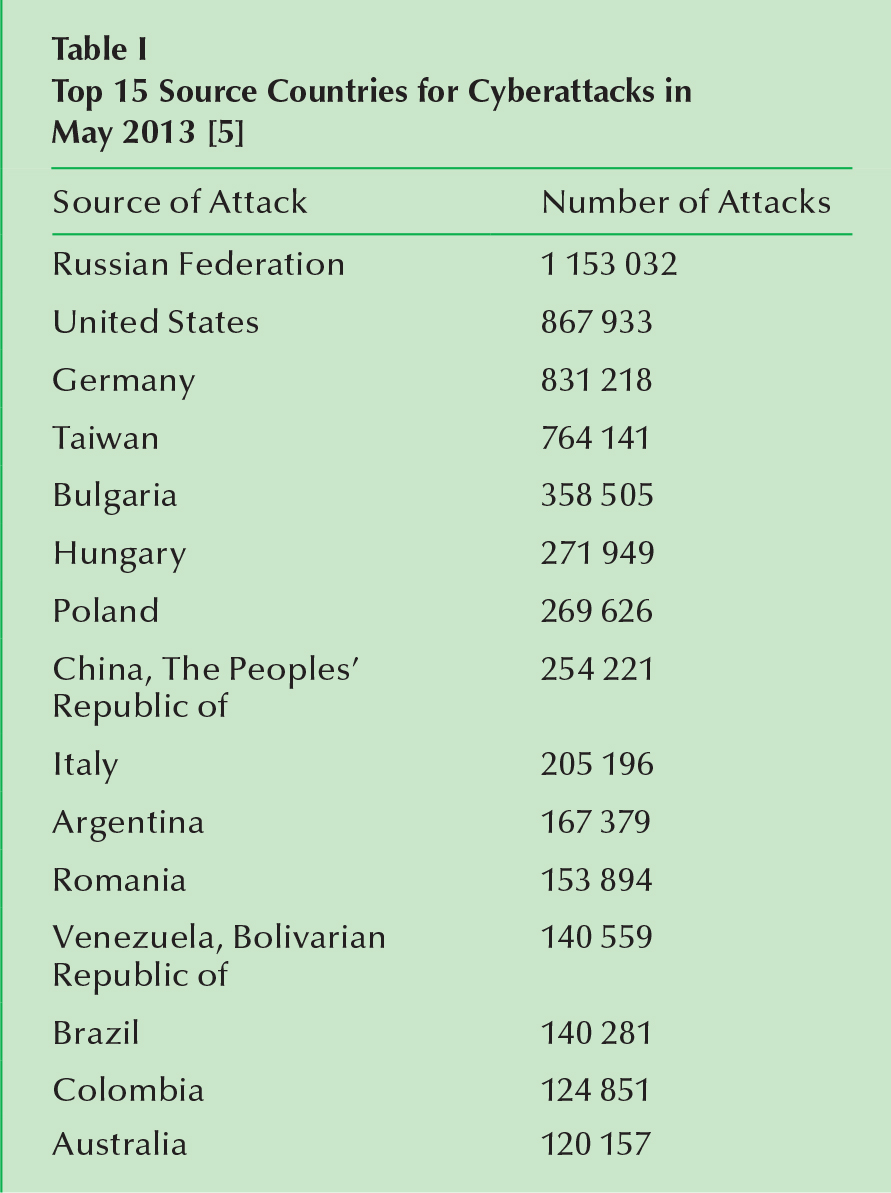
\includegraphics[width=55mm]{slika1.jpg}
  \end{center}
  \caption{Top 15 zemalja izvora za sajber napade u maju 2013. \cite{Overview of current cyber attacks}}
  \label{fig:vr1}
\end{figure}

\newpage

 



\section{Zasto se javlja sajber rat?}
\label{slike_i_tabele}

Za manje drzave ili teroristicke oraganizacije upotreba DDoS (Distributed Denial of Service) napada je mnogo jeftinija(i takodje efikasnija) za pokretanje od konvencionalnih ratnih oruzja i metoda napada protiv naprijatelja, koji uglavnom poseduje veci kolicinu resursa, vojne opreme, vojnih snaga, novca i generalno je veca vojna sila. Samom pojavom sajber rata pojavilo se i novo zanimanje pod nazivom sajber napadac. Sajber napadac za iznajmljivanje je profitabilan posao za one koji su ranije bili samo sajber kriminalci.
Kao sto su primetili mnogi, sajber kriminalci mogu postati sajber ratnici za iznajmljivanje . 
Ovaj lagani prelazak sa sajber kriminala na najam sajber ratnika sugerise to oslanjanje na strogo razgranicavanje između dve aktivnosti.
Sajber kriminal i sajber napadi mogu dugoročno dovesti do povecanja sajber napada.
Sami sajber napadi imaju sposobnost da poremeta nacin zivota obicnoh ljudi(npr. haos koji bi se desio da se izvrsi sajber napad na neki bankomat ili banku i racune u njoj). Takodje medjusobna povezanost globalnih finansijskih institucija povecava rizik za sajber napad.







\section{Kako se javlja sajber rat?}
\label{sec:naslov1}


Prilikom sajber napada koriste se razni vektori, kako tehnosloski tako i orgazicaioni. Napadi traze ranjivost u bilo kom od delova koji cine sajber prostor. Istrazivanjima je otkriveno da je veca verovatnoca da ce odredjene vrste napada poteci iz odredjenih drzava i regiona. Na primer 75 procenata dobavljaca internat usluga koji sadrze najvise phishing prevara posticu iz Sjedinjenih Americkih Drzava.

\begin{verbatim}
\end{verbatim}

\begin{figure}[h!]
  \centering
  \begin{center}
  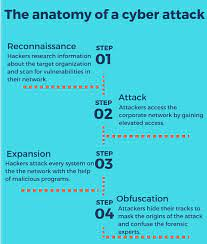
\includegraphics[width=55mm]{index.jpeg}
  \end{center}
  \caption{Slikovito prikazan proces sajber napada.}
  \label{fig:vr1}
\end{figure}

\newpage

\section{Metode napada u sajber prostoru}
\label{sec:naslov2}

 \begin{figure}[h!]
  \centering
  \begin{center}
  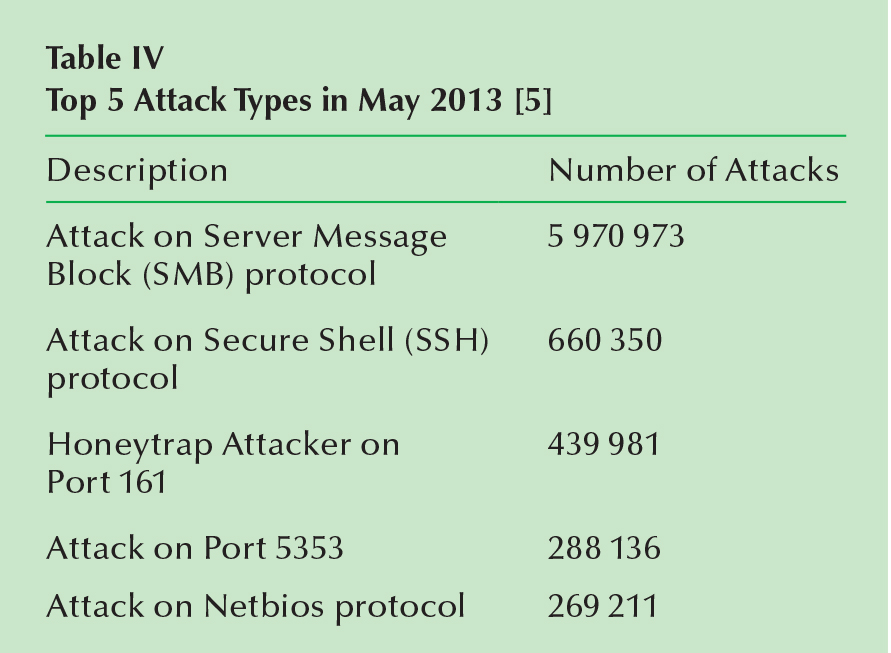
\includegraphics[width=55mm]{slika2.jpg}
  \end{center}
  \caption{Neke od zabelezenih metoda sajber napada}
  \label{fig:vr1}
\end{figure}

Na prikazanoj slici iznad se vidi 5 najpopularnijih vrsta napada otkrivenih u maju 2013te koje je otkrio sistem za identifikaciju napada koji je postavio DTAG. Kao sto se sa slike moze videti vise od 50 procenata ovih napada je na Server Message Block protokolima.
Takodje SCADA sistemi su posebno osetljivi na sajber napade, a time i poprilicno privlacni za sajber napadace. Naime SCADA, ili sistem nadzorne kontrole i prikupljanja podataka se koristi za kontrolu, pracenje i analizu industrijskih uredjaja i procesa.
Sistem se sastoji od softverskih i hardverskih komponenti i omogucava daljinsko prikupljanje podataka kao i prikupljanje na licu mesta. Ovim sistemom se omogucava kompanijama da daljinski upravljaju industrijskim lokacijama kao sto su na primer vetroparkovi itd...
Kako su SCADA sistemi sve vise povezani sa drugim mrezama, ukljucujuci i internet, samo povecavanje sanse za spoljasnju napad se prirodno desava.


\section{Klasifikacija sajber napada}
\label{sec:naslovN}

\begin{figure}[h!]
  \centering
  \begin{center}
  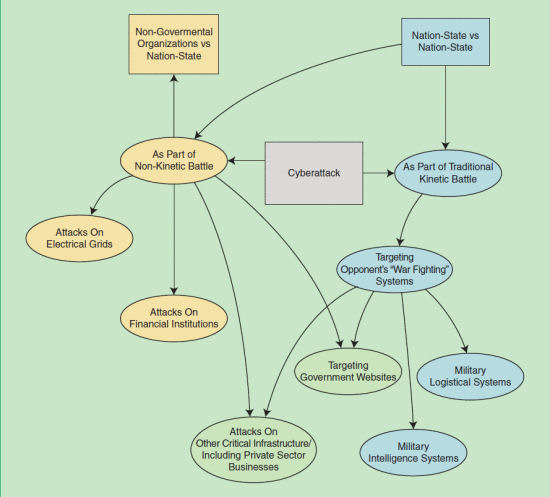
\includegraphics[width=55mm]{proces.jpg}
  \end{center}
  \caption{Proces odvijanja samog napada}
  \label{fig:vr1}
\end{figure}

Sajber napade mozemo podeliti po nivoima pokretanja i nivoima na kojima moze doci do sajber napada:
\begin{itemize}
    \item Vlada naspram vlade (u pogledu kineticke bitke)
    \item Asimetricno ratovanje: nedrzavni akter protiv sopstvenih agencija ili dobavljaca, ili druge vlade (pod nedrzavnim akterom se misli na razne teroristicke grupe, politicke grupe...)
    \item Vlada protiv kriticne infrastrukture druge vlade
    \item  Krivicno nadahnuti hakeri naspram pojedinacnih korisnika
\end{itemize}

Pored ovakve podele mozemo navesti i razlicite vrste napada po kojima ih mozemo podeliti:
\begin{itemize}
    \item Phishing(pecanje) - napadi ove vrste su izuzetno cesti i ukljucuju slanje velikih kolicina lazne elektronske poste na ime nekog pouzdanog izvora (npr. vasa banka). Elektronske poruke cesto izgledaju kao legitimne, ali povezuju primaoca sa zlonamernom datotekom ili skriptom dizajniranom da omoguci napadacima pristup vasem uredjaju.
    \item MitM ili Man in the Middle - ova vrsta napada se javlja kada napadac presrece dvostranu transkaciju, ubacujuci se u sredinu. Odatle sajber napadaci mogu da kradu podatke i da njima manipulisu tako prekidajuci saobracaj. Ova vrsta napada obicno iskoriscava bezbedonosne propuste u mrezi, ko sto je neobezbedjen javni Wi-Fi, da bi se ubacio izmedju uredjaja posetioca i mreze.
    \item Dos ili Denial of Service - ovi napadi funkcionisu tako sto preplavljuju sisteme, servere ili mreze saobracajem radi preopterecenja resursa i propusnog opega. Rezultat ovog napada je sistem koji nije u stanju da obradi ili ispuni zahteve korisnika.
    Pored DoS postoji i DDoS  ili Distributed Denial of Service. DoS napadi prezasicuju sistemske resurse sa ciljem da ometaju odgovor na zahteve korisnika. Sa druge strane DDoS napad se pokrece sa nekoliko zarazenih host masina sa ciljem da se postigne uskracivanje usluge i da se sistem iskljuci.
    \item pored ovih navedenih postoji jos dosta vrsta kao sto su Malware (zlonamerni softveri), SQL injetion itd...
\end{itemize}



\section{Najpoznatiji zabelezeni primeri sajber napada}
\label{sec:naslovM}


Dok je Rusija jos uvek bila u sastavu Sovjetskog saveza 1982. godine, deo njene Trans-sibirskog gasovoda eksplodirao je, navodno zbog implementiranog malvera u piratskoj verziji kanadskog softvera koji je podmetnula CIA. Malver je izazvao malfunkciju u SCADA sistemu koji je pokretao kompletan gasovod.
Hakeri su 2008. godine tokom Gruzijskog rata, odnosno rata u Juznoj Osetiji, obarali Ruske, Osetijske, Gruzijske i Azerbejdzanske sajtove.
Sajber napadi koje su predvodili Rusi:
Postoje tvrdnje da su ruske tajne službe organizivale nekoliko DDoS napada kao deo njigovog sajber ratovanja protiv drugih država, najpoznatiji slucajevi su napad na Estoniju 2007. godine, i na Juznu Osetiju, Gruziju i Azerbejdzan 2008. godine. Jedan od identifikovanih hakera rekao je da je bio placen od strane FSB da vodi hakerske napade na NATO kompjutere. Studirao je informatiku u Sektoru za odbranu informacija.

Iran je bio i zrtva i predator nekoliko operacija sajber ratovanja. Smatra se vojnom silom u procvatu te je stoga interesantna meta ovakvih napada.
Septembra 2010, Iran je napadnut Staksnet crvom, sa namerom da se specificno pogodi nuklearno postrojenje Natanz. To je bio kompjuterski crv od svega 500 kilobajta koji je zarazio 14 industrijskih sajtova u Iranu, ukljucujuci i Natanz postrojenje. Iako pravi tvorci Staksneta nikada nisu identifikovani, smatra se da su ga razvili SAD i Izrael i zajedno ga i pustili u pogon. Taj crv je, smatra se, najnapredniji komad malvera ikada otkriven i značajno je uticao na poimanje opasnosti sajber ratovanja.
U ratu protiv Hezbolaha 2006 godine, Izrael tvrdi da je doslo do sajber ratovanja tokom sukoba. Obavestajne službe Oruzanih snaga Izraela su dosli do podataka da je nekoliko zemalja na Bliskom istoku unajmilo ruske hakere i naucnike da rade za njih. Kao rezultat toga Izrael je posvetio posebnu paznju sajber taktici i postao time, jedna od jedinih drzava u svetu, pored SAD, Francuske i jos nekoliko zemalja, koja se bavi planiranjem za sajber rat. Mnoge međunarodne IT kompanije se sele i pocinju da istrazuju podrucje Izraela. Ricard Klark dodaje da su "naci izraelski prijatelji naucili ponesto o programima na kojima mi radimo vec dve decenije."
Septembra 2007. godine, Izrael je izvrsio vazdusni napad na Siriju. Namenska industrija SAD kao i vojni izvru spekulisu da su izraelci mozda koristili sajber ratovanje kako bi omogućili svojim avionima da prodju neopazano sirijski radar.
\section{Sajber napadi u Srbiji}

Srbija se u junu 2021. godine nasla na sedmom mestu globalne liste zemalja po broju napada na industrijske racunare, prema podacima kompanije "Kaspersky". Prema podacima RATEL-a na svakih 39 sekundi desi jedan sajber napad u našoj zemlji.
Problemi u vezi sa hakerskim napadima sve su cesci kako u svetu, tako i u Srbiji, zato sto postajemo sve zavisniji od tehnologije. Naime, sto je jedna država razvijenija i sto vise koristi naprednu tehnologiju postaje ranjivija i ugroženija od sajber napada.
Eksperti za ovu oblast navode da je jedan od glavnih problema slab mehanizam odbrane, ali  oni dodaju da napredak u Srbiji postoji. 
Istrazivanje koje je sprovedeno u 69 gradova i opstina u Srbiji pokazuje da 58 posto lokalnih samouprava nije proveravalo bezbednost mreze, a niko od anketiranih nije u poslednjih godinu dana testirala plan oporavka u slucaju kolapsa sistema. Dok takodje postoji podatak da 47\% lokalnih samopurava bilo meta sajber napada, a 12\% ni ne zna da su bili napadnuti.  

\addcontentsline{toc}{section}{Literatura}
\appendix

\iffalse
\bibliography{seminarski} 
\bibliographystyle{plain}
\fi

\begin{thebibliography}{9}

\bibitem{Cyberwar} Angelyn Flowers, Sherali Zeadally, Cyberwar: The What, When, Why, and How
  Article in IEEE Technology and Society Magazine · September 2014,
  https://technologyandsociety.org/cyberwar-the-what-when-why-and-how/

\bibitem{DCAF Horizons} F. Schreier, On Cyberwarfare: DCAF Horizons 2015 Working
Paper. Geneva: Defense Center for Armed Forces, 2013.

\bibitem{Cyberwar thresholds and effects} J. Lewis, “Cyberwar thresholds and effects,” IEEE Security and
Privacy, pp. 23–29, Sept./Oct. 2011.

\bibitem{Declarations of cyberwar} W. Jones, “Declarations of cyberwar: What the revelations about
the U.S.-Israeli origin of Stuxnet mean for warfare,” IEEE Spectrum,
pp. 18, Aug. 2012

\bibitem{Overview of current cyber attacks}Deutsche Telekom AG, “Overview of current cyber attacks;” http://
www.sicherheitstacho.eu/, accessed June 6, 2013.

\bibitem{The Threat in Cyberspace} R. O’Harrow, Jr., Zero Day: The Threat in Cyberspace. New York,
NY: Diversion Books, Washington Post E-Book, 2013.

\bibitem{Improving critical infrastructure cybersecurity}B. Obama, “Executive order 13636: Improving critical infrastruc-
ture cybersecurity,” Federal Register, vol. 78, no. 33, part III, Feb.19,
2013.

\bibitem  Sajber rat Vikipedija

\bibitem https://www.euronews.rs/srbija/drustvo/25537/jedan-sajber-napad-na-svakih-39-sekundi-srbija-u-vrhu-po-broju-hakerskih-upada/vest


\end{thebibliography}

\end{document}
